\documentclass[a4paper, 11pt]{article}
\usepackage[left=2.5cm,right=2.5cm,top=3cm,bottom=3cm,a4paper]{geometry}
\usepackage{kotex}
\usepackage{color}
\usepackage{enumitem}
\usepackage{graphicx,subfigure}
\DeclareGraphicsExtensions{.pdf,.png,.jpg}




\title{\textbf{\Huge오목 한글 설명서}}
\author{\textbf{\LARGE5조}}
\begin{document}
   
   \maketitle
   
   \vspace{6cm}
\begin{center}
   \textbf{\large20134824김민석}\\
   \textbf{\large20134852허정건}\\
   \textbf{\large20134867이현문}\\
\end{center}
   
   
   
   
   \maketitle
   \newpage
   \thispagestyle{empty}        
   \mbox{}
   
   \begin{center} 
      \textbf{\Huge목차}\\
   \end{center}
   \vspace{1cm}
   \section{프로그램 채택 이유}
   \vspace{1cm}
   \section{프로그램 설명}
   \vspace{1cm}
   \section{사용 설명}
   \vspace{1cm}
   
   \section{기능 설명}
   \begin{enumerate}
      \item a설명
      \item b설명
      \item c설명

   
   \end{enumerate}

   

   
   \vspace{1cm}
   \section{버그와 개선할점}
   
   \vspace{1cm}
   \section{느낀점}
   
   
	\newpage
	\title{\textbf{\Huge1. 프로그램 채택 이유}}
	\\
   \ 다들 한번쯤 간단한 콘솔게임을 많이 해보셨을꺼라고 생각합니다. 그중 대표적인 게임으로 시작프로그램에 있는 윈도우즈용 간단한 게임들인 스파이더맨,지뢰찾기,프리쉘 등등 많이 있습니다. 하지만 최근 os가 윈도우10으로 바뀌면서 시작프로그램의 지뢰찾기등 많은 간단한 게임 프로그램들이 사라졌습니다. 저희는 이런 옛 추억적이고 학창시절 친구들과 자주했던 게임들중 여러개중 하나인 오목을 선택하게 되었습니다.
   
   
   
   \newpage
   \title{\textbf{\Huge2. 프로그램 설명}
   	\\ 이 콘솔프로그램은 네이버 어느유저가 올린 오픈소스프로그램으로써 간단한 오목을 즐기는 프로그램이다. 
   	
   	게임 방식 으론 키보드 방향키와 스페이스를 사용하여 가로, 세로 대각선으로 같은 색 알을 다섯 개 먼저 늘어놓으면 승리하는 게임으로, 상대방의 돌이 다섯 개가 되기 전에 라인 양 끝을 막여 것으로 방어한다. 
   
   
   
   \newpage
   \title{\textbf{\Huge4. 게임 룰 설명 및 조작법 }
   	\vspace{0.5cm}
   
 	\quad1)게임룰
 	\begin{figure}[h]
 		\begin{center}
 			\subfigure{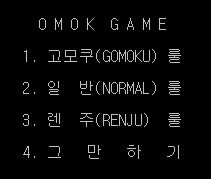
\includegraphics[width=0.35\linewidth]{OM_RuleSELECT.png}}
 			 			\\ 오목게임실행시 첫 화면으로 고모쿠룰 일반룰 렌주룰 3가지중 하나의 룰을 선택합니다.
 			\vspace{3.2cm}  	
 			    \begin{flushleft}
 			    	\qquad1.1)고모쿠 룰	
 			    \end{flushleft}
 			
 			
 			\subfigure{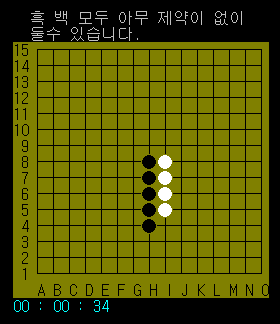
\includegraphics[width=0.35\linewidth]{komoku.png}}
 			
 				
 			\begin{flushleft}
 				\ 아무런 제약이 없는 오목으로, 먼저 두는 흑돌 에게 유리하다. 백돌 에게 불공평하기 때문에 공식에서 잘 쓰이지 않는다. 
 			\end{flushleft}
 		\end{center}
 	\end{figure}
 
 	
 	
 	
 	\newpage
	\quad1.2)일반룰
        \begin{figure}[h]
    	\begin{center}
    			\subfigure{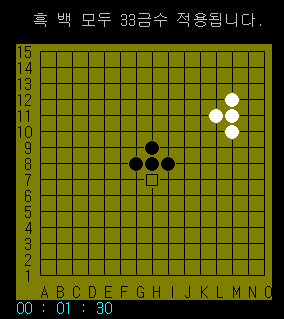
\includegraphics[width=0.30\linewidth]{normal.png}}
    			
    		\ \begin{flushleft}
    			일반룰 : 일상적으로 가볍게 대전할 때 가장 많이 사용되는 룰이다. 일단 3-3은 흑, 백 모두 금지되나 여기서 2개의 라인의 양 끝, 즉 4개의 끝 중 하나라도 막혀있으면 금지수가 아니다. \qquad 4-4에서 4가 하나 띄워져 있더라도 금지이다.
    		\end{flushleft}
    		
    		\vspace{2cm} 	
    			
    		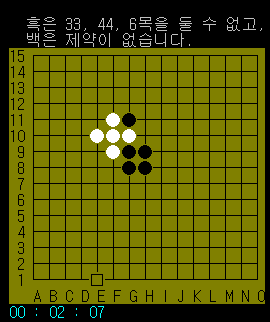
\includegraphics[width=0.35\linewidth]{renju.png}
    		\\ 렌주룰 : 흑만 3-3, 4-4가 금지된다. (단, 4 또는 3과 동시에 5도 만들 수 있는 상황이라면 가능하다)
    	\end{center}
    \end{figure}


  
  
  \newpage
  \title{4.2 게임조작법} \\
  
  
  \begin{figure}[h] %%% t: top, b: bottom, h: here
  	\begin{center}
  		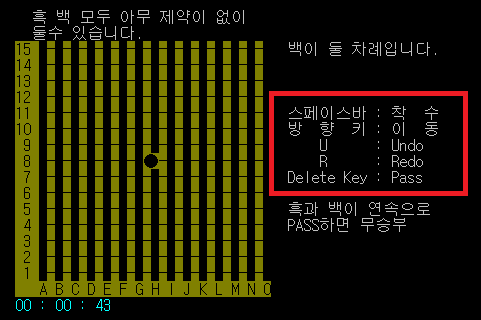
\includegraphics[width=0.7\linewidth]{OM_5.png}
  	\end{center}
  	\vspace{0.5cm}
  
  
  
  4.2.1 스페이스바 \\
 \qquad내 차례일 경우, 원하는 위치에 스페이스바를 눌러 착수\\

  4.2.2 방향키 \\
  \qquad↑ : 위쪽으로 한칸 이동 \\
  \qquad↓ : 아래쪽으로 한칸 이동 \\
  \qquad← : 왼쪽으로 한칸 이동 \\
  \qquad→ : 오른쪽으로 한칸 이동 \\
  
  4.2.3 U \\
  \qquad이미 착수된 돌을 다시 되돌리는 기능\\
  
  4.2.4 R \\
  \qquad다시 두고 싶을 때 이미 착수된 돌을 되돌리는 기능\\ 
      
  4.2.5 Delete Key \\
  \qquad 내 턴을 무시하고 다음 턴으로 넘기는 기능 \\
  \end{figure}
  
\end{document} 